\begin{figure}
  \centering
  \begin{subfigure}[b]{0.3\textwidth}
    \centering
    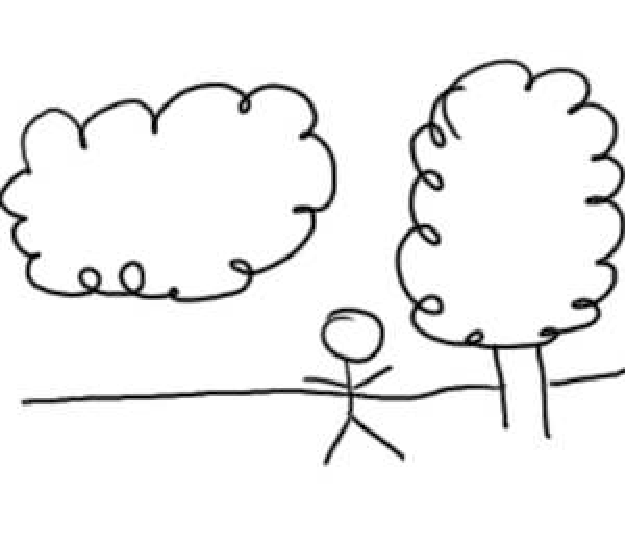
\includegraphics[width=\textwidth]{img/cloud-1.pdf}  
    \caption{Overloaded semantics: The cloud and tree have similar
             shapes but different meanings due to context.}
    \label{fig:cloud-1} 
  \end{subfigure}
  \hspace{0.03\linewidth}
  \begin{subfigure}[b]{0.3\textwidth}
    \centering
    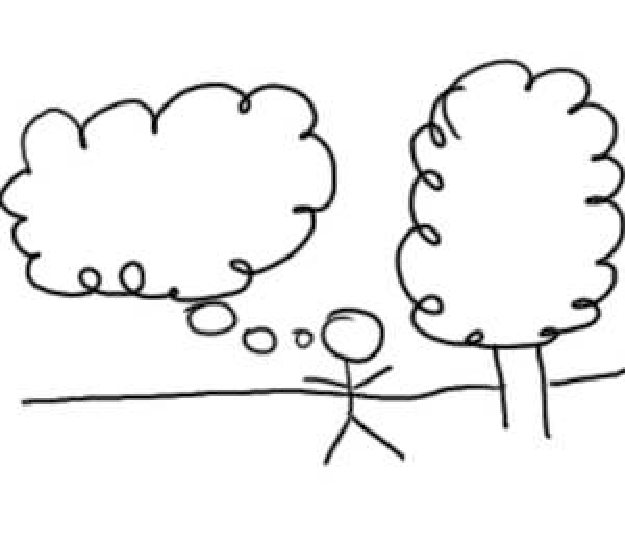
\includegraphics[width=\textwidth]{img/cloud-2.pdf}  
    \caption{Ambiguity: A small addition changes our
      interpretation. The object at left may be a cloud or a thought
      bubble.}
    \label{fig:cloud-2} 
  \end{subfigure}
  \hspace{0.03\linewidth}
  \begin{subfigure}[b]{0.3\textwidth}
    \centering
    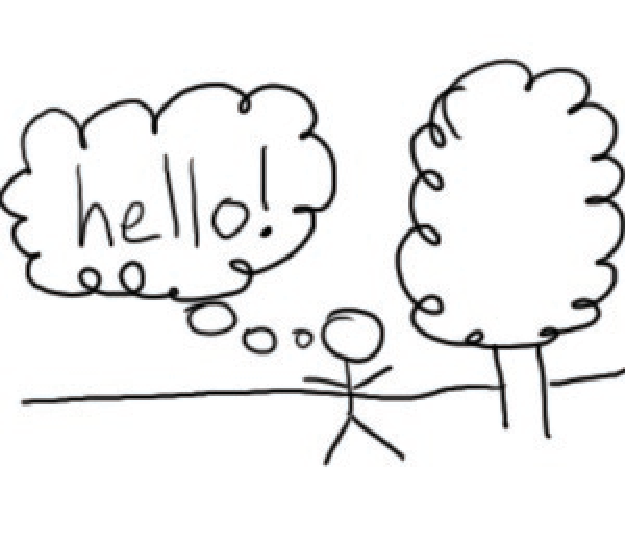
\includegraphics[width=\textwidth]{img/cloud-3.pdf}  
    \caption{More information gives more confidence about object
      identity. Text in the cloud indicates a thought bubble.}
    \label{fig:cloud-3} 
  \end{subfigure}

  \caption[Overloaded semantics and ambiguity]{Overloaded semantics
    and ambiguity.}
  \label{fig:cloud}
\end{figure}
